\section{Achievements of Deep Learning}
Deep Learning has had an explosion in applications and research and development
for the last decade. These applications include:

\begin{itemize}
    \item Automatic speech recognition
    \item Image recognition
    \item Visual art processing
    \item Natural language processing
    \item Drug discovery and toxicology
    \item Customer relationship management
    \item Recommendation systems
    \item Bioinformatics
\end{itemize}

The theoretical foundations of the field is old (mid 19th century), but the 
playground for these algorithms has just now arrived. These include large
datasets, computational hardware and software. 

\section{Comparison with traditional machine learning}
In traditional machine learning development. One needs domain knowledge for
developing good models. Domain knowledge let's you select good features 
and good features give good models. One example could be a certain visual
feature in a certain kind of biomedical image. This field is called 
\textbf{feature engineering}. 

\section{Feature Learning}
Feature Learning, also known as \textbf{Representation Learning} is a set of
techniques that allow systems to automatically discover the representation 
needed for feature detection or classification. Feature learning methods 
let us replace the manual feature engineering that is done in traditional 
machine learning development. A lot of deep learning architectures for 
representation learning have been researched and published in the last decade.

\section{Motivations for deep learning}

Deep Learning let's us model nonlinear decision boundaries by introducing
nonlinearities in the activation functions and deep architectures. This means 
that deep learning is especially fit for problems that are too complex for 
linear methods. One could question wether models like logistic regression could
be used with polynomial decision boundaries to achieve the same thing. 
The problem with using regression is that it achieves this by introducing
polynomial features. The number of features the model must take into account
is then 

\begin{equation*}
    \sum_{i = 1}^k \binom{k + i - 1}{i} = \binom{k+n}{n} - 1
\end{equation*}

where $n$ is the polynomial degree that you want the model to incorporate and
$k$ is the number of features/variables. \cite{mathoverflowquestion}
For $100$ features, introducing $k = 2$ gives over 5000 features. This is not
feasible. 

\section{Artificial Neuron}
\begin{itemize}
    \item Feed input via input nodes
    \item Logistic unit does some computation
    \item Sends output
\end{itemize}

\bigskip
\begin{figure}[H]
\centering
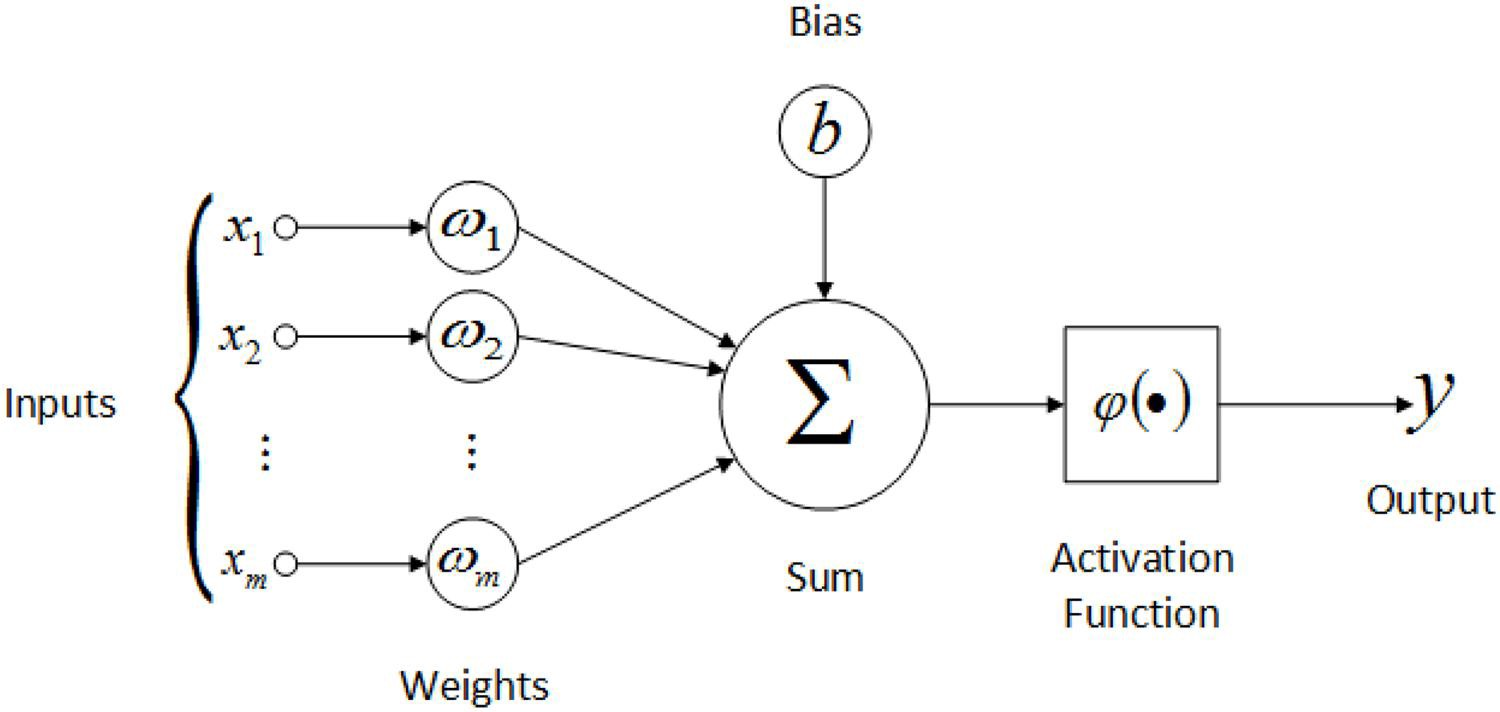
\includegraphics[scale=0.25]{figures/artificialneuron.jpeg}
\caption{Artificial Neuron}
\end{figure}

The activation function is typically the sigmoid function, a hyperbolic tangent, 
or a rectified linear unit (ReLU). They must be a non-linear function because
several layers of linear activation functions still yield a linear decision 
boundary. Deep layers of non-linear activations yield complex decision
boundaries.

\section{Notations}
\begin{itemize}
    \item $a_i^{(j)}$ - Activation of unit $i$ in layer $j$ (the output of the node)
    \item $\theta^{(j)}$ - Matrix of parameters (controlling the activation from one layer to the next)
    \item $g(\theta^Tx)$ - The activation function
\end{itemize}

\section{Multiclass Classification}
\begin{itemize}
    \item Given $N$ classes:
    \begin{itemize}
        \item Build a neural network with $N$ output units
        \item Use one-hot encoding to encode the output as an array of $N-1$ zeros and one $1$.
    \end{itemize}
\end{itemize}

\section{Cost function for Neural Networks}
The cost function can generate $k$ outputs, meaning that the sigmoid function (or any other cost functions) returns a $k$ dimensional vector.

The cost function is combined by two parts.

\bigskip

The first part finds the mean of the sum of each training sample $m$, over the sum of each class $k$. All classes has a "one-vs-all" comparison. This gives the following expression:

\[
    -\frac{1}{m}\left[\sum_{i=1}^m\sum_{k=1}^Ky_k^{(i)} \log\left(h_\Theta(x^{(i)})\right)_k+(1-y_k^{(i)}) \log\left(1-(h_\Theta(x^{(i)}))_k\right)\right]
\]

The second part is the regularization term. In this part, we sum all layers $L-1$, over all units in each layer $s_t$, over all the input layers $j$:

\[
    \frac{\lambda}{2m}\sum_{l=1}^{L-1}\sum_{i=1}^{s_t}\sum_{j=1}^{s_l+1}(\Theta_{ji}^{(l)})^2
\]

\section{How to minimise the cost function}

To minimise the cost function, we need to change the weights and biases of the 
neural network such that this cost function is decreased. This is achieved using
calculus and gradient descent. Recall from calculus that the gradient can be
interpreted as the direction and rate of fastes increase. In gradient descent
one therefore wish to iteratively go opposite to the gradient to reach a minima.
When performing gradient, convergence to a local minima is guaranteed. 
When the cost function is convex, all local minima is also global minima.
The nature of the cost function is therefore important to consider. 
Global optimisation is a field of mathematics concerning this and there exists 
many deterministic and stochastic methods to achieve this.

\section{Gradient Descent}
Here, we will focus on gradient descent as a way to achieve minima. Consider the
following algorithm:

\begin{algorithm}[H]
    \SetAlgoLined
    \KwResult{Local og global minima}
    Initialise $\theta \sim N(0, \sigma^2)$, $\epsilon$, $\alpha$.

    \While{$\Delta J > \epsilon$}{
        Compute gradient $\frac{\partial J(\theta)}{\partial \theta}$\;
        Update weights $\theta = \theta - \alpha \frac{\partial J(\theta)}{\partial \theta}$\;
    }

    Return $\theta$
    \caption{Gradient Descent}
\end{algorithm}

This is a general algorithm for the intuition behind gradient descent. But how 
do we achieve this for the multivariate case with several layers of activation?
Let us introduce \textbf{backpropagation}

\section{Backpropagation}

When calculating partial derivatives for a neural network. One starts at the
output layer and calculate the derivatives backwards. 
One begins by calculating the error between the activations of the output and 
the true state of nature.

\begin{equation*}
    \delta^{(L)} = a^{(L)} - y
\end{equation*}

then compute 

\begin{equation*}
    \delta^{(L-1)} = (\theta^{L-1})^T\delta^{(L)} \cdot g'(z^{(L-1)})
\end{equation*}

and do this until we reach layer $1$.

\section{Hyperparameters and model enginnering}

After understanding gradient descent, backpropagation, activation function etc,
one is ready to start to engineer neural networks for ones needs. But there is 
one problem, the hyperparameters. In this section some of these hyperparameters
and challenges will be discussed.

\subsection{Loss Functions in reality}

These are very seldom convex. One may be able to change the loss function 
to make it more convex, but this may not work. Evolutionary and stochastic
algorithms that explore the loss function space may help. Selecting losses
and ensuring that these are well behaved is a challenge when creating neural
networks.

\subsection{Initialisation of weights}

Weights must be initialised and these must be initialised using a gaussian
distrubution with mean at $0$. 

\subsection{Learning Rate}
Learning rate is a model hyperparameter that must be considered. If learning 
rate is too low, the model does not explore the cost function space and
converges in local minima. If it is too large, it may diverge and cause
the exploding gradient problem. Learning rates may be changed over time
and so on.

\subsection{Mini-batches}
Instead of computing gradients for individual samples, batches may be used 
instead. This gives a smoother convergence and allows for larger learning
rates. This also allows for parallelising comutation!

\subsection{Overfitting and regularisation}
Neural networks have a quite large hypothesis space and capacity. This allows 
them to quickly overfit. Large amounts of data is needed to make to model
generalisable. Regularisation may also help by introducing a penalty for 
complexity. Dropout is a much used way to regularise neural networks.
It simply removes nodes from the neural network during a training step and
forces the model to learn using a smaller capacity.

\medskip

Early stopping is also an alternative, by using learning curves one should stop
the training as soon as one observes that the accuracy of the testing set is 
getting worse compared to the training accuracy.